\begin{question}
  \hspace*{\fill} [Note maximale: 6]\par
  \medskip
  \begin{center} % or flushleft or flushright
    \noindent Le diagramme suivant est la représentation graphique de la fonction $f(x)$ pour $ -4 \le x \le 2$.\par
    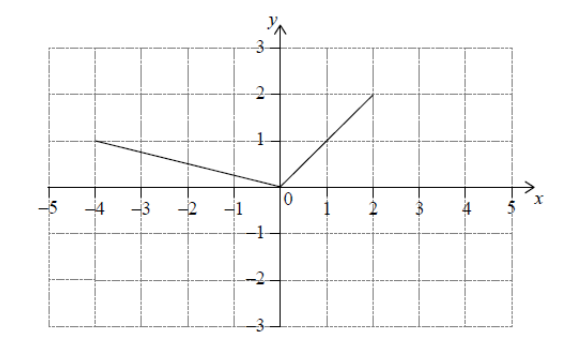
\includegraphics[scale=0.4]{diagramme_x1a}\par
    \noindent Diagramme A\par
  \end{center} % or flushleft or flushright
  \medskip
  \begin{center} % or flushleft or flushright
    \noindent Une autre fonction, $g$, peut s’écrire sous la forme $g(x) = a \times f(x + b)$. Le diagramme suivant
montre la représentation graphique de g.\par
    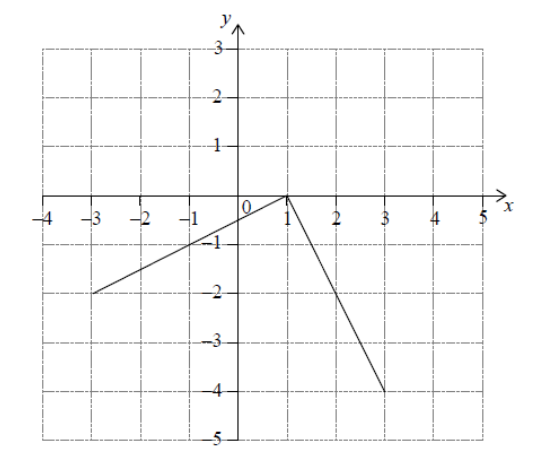
\includegraphics[scale=0.4]{diagramme_x1b}\par
    \noindent Diagramme B\par
  \end{center} % or flushleft or flushright
  \medskip
  % Question broken down into a list of parts each with its component maximum mark
  \begin{enumerate}[label=(\alph*)]
    \item Sur le système d'axes du diagramme A esquissez la représentation graphique de f(-x)\hspace*{\fill} [2]
    \item Selon le diagramme B, écrivez la valeur de $a$ et de $b$ de la fonction $g$ \hspace*{\fill} [4]
  \end{enumerate}
\end{question}
